\begin{surferPage}[Altıgil (30 Gaga)]{Barth'ın 30 Gagalı Altıgili}
Wolf Barth'ın olası en fazla ($65$) tekilliğe sahip altıgili (galeride diğer bir resim)
inşa etmesinin  ve kendisinin iki doktora öğrencisinin daha yüksek dereceler için yeni dünya rekoru yüzeyleri bulmalarının ardından, Barth derecesi verilen bir yüzeyde bulunabilecek en fazla gaga tekilliği sayısı üzerinde çalışmaya başladı.

   Barth'ın $A_1^{+-}$ (yani çift koni) tekilliklerinden  $65$ adet ürettiği inşası gaga tekilliklere de uyarlanabilir. Barth'ın Altıgilinde olduğu gibi $P_6$ yirmiyüzlünün simetri düzlemlerini ve $K$ yine bir birim küreyi göstermek üzere,
    \[P_6 - \alpha \cdot K^3=0\]
ifadesi $30$ adet gaga tekilliği verir:
    \vspace*{-0.4em}
    \begin{center}
      \begin{tabular}{c@{\ }c@{\ }c@{\ }c}
        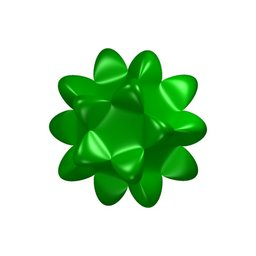
\includegraphics[height=1.2cm]{./../../common/images/barthsextic_30A2}
        &
        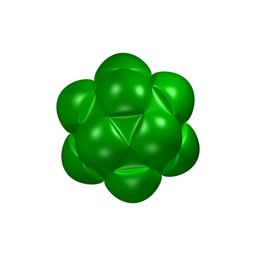
\includegraphics[height=1.2cm]{./../../common/images/barthsextic_30A2_3}
        &
        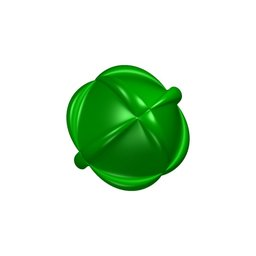
\includegraphics[height=1.2cm]{./../../common/images/barthsextic_30A2_5}
        &
        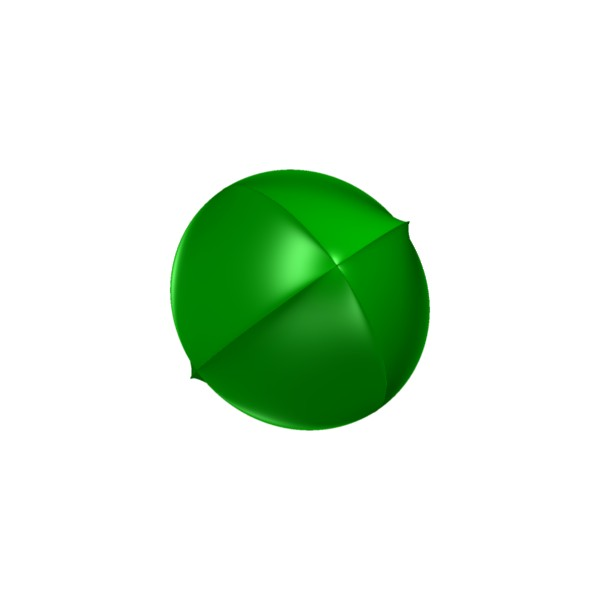
\includegraphics[height=1.2cm]{./../../common/images/barthsextic_30A2_6}
      \end{tabular}
    \end{center}    
    \vspace*{-0.3em}
 Bu, altıgiller üzerinde gerçel gaga tekillik sayısı için şu anki dünya rekorudur. Kompleks gagalar için bu sayı $36$'dır.
\end{surferPage}
